%% This is file `DEMO-TUDaExercise.tex' version 2.10 (2020/04/26),
%% it is part of
%% TUDa-CI -- Corporate Design for TU Darmstadt
%% ----------------------------------------------------------------------------
%%
%%  Copyright (C) 2018--2020 by Marei Peischl <marei@peitex.de>
%%
%% ============================================================================
%% This work may be distributed and/or modified under the
%% conditions of the LaTeX Project Public License, either version 1.3c
%% of this license or (at your option) any later version.
%% The latest version of this license is in
%% http://www.latex-project.org/lppl.txt
%% and version 1.3c or later is part of all distributions of LaTeX
%% version 2008/05/04 or later.
%%
%% This work has the LPPL maintenance status `maintained'.
%%
%% The Current Maintainers of this work are
%%   Marei Peischl <tuda-ci@peitex.de>
%%   Markus Lazanowski <latex@ce.tu-darmstadt.de>
%%
%% The development respository can be found at
%% https://github.com/tudace/tuda_latex_templates
%% Please use the issue tracker for feedback!
%%
%% ============================================================================
%%
% !TeX program = lualatex
%%

%=========================================================

% Here you can choose to compile with or without solutions.
% However, this definition is ignored if you use any
% command from the `Makefile`.
%\providecommand{\withSol}{\iftrue}

%=========================================================
\documentclass[
	ngerman,
	colorback=false,
	solution=true,
	]{tudaexercise}

\usepackage[english, main=ngerman]{babel}
\usepackage[babel]{csquotes}
\usepackage{amsmath}
\usepackage{booktabs}
%~~~~~~~~~~~~~~~~~~~~~~~~~~~~~~~~~~~~~~~~~~~~~~~~~~~~~~~~~
% Zusätliche Pakete
\usepackage{comment}
\newcommand{\urlc}[1]{\color{cyan}\url{#1}\color{black}}
\newcommand{\hrefc}[2]{\color{cyan}\href{#1}{#2}\color{black}}
\newcommand{\prog}[1]{\textit{#1}}
\newcommand{\concept}[1]{\textbf{#1}}
\newcommand{\codesym}{\textbf{\texttt{</>}}}
\usepackage{cite}
\usepackage{dirtree}
\usepackage{amssymb}
\usepackage{tikz}
\usepackage{textcomp}
\usepackage{url}
\usepackage[newenum]{paralist}
\usepackage{bbding}

% The (in)famous algorithm package
\usepackage[vlined,linesnumbered]{algorithm2e}
\SetArgSty{textnormal}
\SetCommentSty{textit}
\usepackage{wrapfig}
\usepackage{nicefrac}
\usepackage{multicol}
\usepackage{multirow}

% Write `B+-tree' consistently throughout the lecture
\newcommand{\Btree}{B\raisebox{.4em}{\textsmaller{+}}-tree}
\newcommand{\Btrees}{B\raisebox{.4em}{\textsmaller{+}}-trees}
\newcommand{\BTree}{B\raisebox{.4em}{\textsmaller{+}}-Tree}
\newcommand{\BTrees}{B\raisebox{.4em}{\textsmaller{+}}-Trees}
\newcommand{\BBaum}{B\raisebox{.4em}{\textsmaller{+}}-Baum}
\newcommand{\BBaums}{B\raisebox{.4em}{\textsmaller{+}}-Baums}
\newcommand{\BBaeume}{B\raisebox{.4em}{\textsmaller{+}}-Bäume}
\newcommand{\R}[0]{\mathds{R}} % real numbers
%~~~~~~~~~~~~~~~~~~~~~~~~~~~~~~~~~~~~~~~~~~~~~~~~~~~~~~~~~

%\usepackage{biblatex}
%=========================================================

\def\homework{7}
\def\homeworkVer{1}
\def\homeworkSolVer{1}
%=========================================================

%Formatierungen für Beispiele in diesem Dokument. Im Allgemeinen nicht notwendig!
\let\file\texttt
\let\code\texttt
\let\pck\textsf
\let\cls\textsf
\let\tbs\textbackslash

\ConfigureHeadline{
	headline={title-name-id}
}

%compatbilitx
\let\unit\relax

\begin{document}

\title[Übungsblatt \homework, Data Mining und Maschinelles Lernen]{Data Mining und Maschinelles Lernen}
\author{Prof. Kristian Kersting\\Zhongjie Yu\\Johannes Czech\\
}
\term{Sommersemester 2021}
\date{\today}
\sheetnumber{\homework}
\setcounter{section}{\homework}

\maketitle
\centering{Diese Übung wird am \textbf{01.07.2021} um \textbf{13:30 Uhr} besprochen und \textbf{nicht bewertet}.}

\begin{table}[h!]
\centering
\begin{tabular}{c|c|c|c|c|c|c|c|c}
\toprule
\textbf{Aufgabe}              & 1  & 2  & 3  & 4 & 5 \\ \hline
\textbf{Maximal Punktzahl}    & 16 & 15 & 19 & 6 & 7  \\ \hline
\textbf{Erreichte Punktzahl}  &   &   &   &   &    \\
\bottomrule
\end{tabular}
\end{table}

\flushleft

\par \textbf{Benötigte Dateien}\\
Alle benötigten Datensätze und Skriptvorlagen finden Sie in unserem Moodle-Kurs: \urlc{https://moodle.informatik.tu-darmstadt.de/course/view.php?id=1058}

\textbf{Theoretische Aufgaben}\\
Bei diesen Übungsaufgaben können Sie Ihren Lösungsvorschlag in \LaTeX~formatieren.
Nutzen Sie hierfür die \LaTeX-Vorlage und die vorgesehene Blöcke.
\begin{verbatim}
\begin{solution}
% Geben Sie hier Ihre Antwort an.
\end{solution}
\end{verbatim}

%\newpage
\begin{task}[credit=16]{Entscheidungsbäume - ID3 Algorithmus}
Die folgende Tabelle zeigt die Entscheidung, ob Baseball gespielt wird, basierend auf vier Wetterattributen.

\begin{table}[h]
\centering
\caption{Trainingsdatensatz, ob Baseball gespielt wird basierend auf der Wetterlage.}
\label{tab:data_baseball}
\begin{tabular}{l|c|c|c|c|c}
\toprule
\textbf{Tag} & \textbf{Ausblick (A)} & \textbf{Temperatur (T)}  & \textbf{Luftfeuchtigkeit (L)} & \textbf{Wind (W)}     & \textbf{Spielt Baseball (B)} \\
\midrule
T1  & Sonnig    & Warm        & Hoch             & Schwach  & Nein            \\
T2  & Sonnig    & Warm        & Hoch             & Stark    & Nein            \\
T3  & Bewölkung & Warm        & Hoch             & Schwach  & Ja              \\
T4  & Regen     & Mild        & Hoch             & Schwach  & Ja              \\
T5  & Regen     & Kühl        & Normal           & Schwach  & Ja              \\
T6  & Regen     & Kühl        & Normal           & Stark    & Nein            \\
T7  & Bewölkung & Kühl        & Normal           & Stark    & Ja              \\
T8  & Sonnig    & Mild        & Hoch             & Schwach  & Nein            \\
T9  & Sonnig    & Kühl        & Normal           & Schwach  & Ja              \\
T10 & Regen     & Mild        & Normal           & Schwach  & Ja              \\
T11 & Sonnig    & Mild        & Normal           & Stark    & Ja              \\
T12 & Bewölkung & Mild        & Hoch             & Stark    & Ja              \\
T13 & Bewölkung & Warm        & Normal           & Schwach  & Ja              \\
T14 & Regen     & Mild        & Hoch             & Stark    & Nein            \\
\bottomrule
\end{tabular}
\end{table}

\begin{table}[h!]
\centering
\caption{Vorhersage-Datensatz, ob Baseball gespielt wird.}
\label{tab:data_baseball_predict}
\begin{tabular}{l|c|c|c|c|c}
\toprule
\textbf{Tag} & \textbf{Ausblick (A)} & \textbf{Temperatur (T)}  & \textbf{Luftfeuchtigkeit (L)} & \textbf{Wind (W)}     & \textbf{Spielt Baseball (B)} \\
\midrule
T15 & Sonnig    & Mild        & Hoch     & Schwach & ?       \\
T16 & Bewölkung & Mild        & Normal   & Schwach & ?       \\
T17 & Regen     & Kühl        & Normal   & Stark   & ?       \\
\bottomrule
\end{tabular}
\end{table}

Die Aufgabe ist es folgende Frage zu beantworten: \textit{Unter welchen Bedingungen wir Baseball gespielt?}

\begin{subtask}[points=10,title=ID3 Algorithmus]
\label{q:id3_alg}
Erstellen Sie den Entscheidungsbaum mittels des ID3 Algorithmus.
Berechnen Sie dabei die \textbf{Entropie} und den \textbf{Informationsgewinn} (engl. \textit{gain}) der Attribut-Selektion für jeden Schritt.
Verwenden Sie bei der Berechnung der Entropie den Logarithmus zur Basis 2, Logarithmus-Dualis.

\textbf{Hinweis:} Sie können \textbf{Spielt Baseball (B)} mit $B$ kennzeichnen. Der Informationsgewinn ist nach Vorlesung wie folgt definiert:
\textit{Differenz zwischen den Informationen der Beispiele mit und ohne die Aufteilung durch $X_j$.}

Bsp. Informationsgewinn für Aufteilung des Wurzelknotens nach dem Merkmal \textit{Ausblick}. 
\begin{align*}
Gain\left (B, Ausblick \right ) &= Entropy\left (B \right ) \\&- \frac{B_\text{Ausblick=Sonnig}}{B}\cdot Entropy\left (B_\text{Ausblick=Sonnig} \right ) \\
&- \frac{B_\text{Ausblick=Regen}}{B}\cdot Entropy\left (B_\text{Ausblick=Regen} \right )\\ &- \frac{B_\text{Ausblick=Bewölkung}}{B}\cdot Entropy\left (B_\text{Ausblick=Bewölkung} \right )
\end{align*}

\begin{solution}
% Geben Sie hier Ihre Antwort an.
\end{solution}
\end{subtask}

\begin{subtask}[points=3,title=Visualisierung]
Erstellen Sie eine Visualsierung (Plot oder eingefügte Zeichnung) des Entscheidungsbaumes aus Aufgabenteil~\ref{q:id3_alg}.

 \begin{solution}
% Geben Sie hier Ihre Antwort an.
\end{solution}

\end{subtask}

\begin{subtask}[points=3,title=Vorhersage]
Geben Sie anhand ihres Entscheidungsbaumes eine Vorhersage für die Tage 15 bis 17 aus Tabelle~\ref{tab:data_baseball_predict}, ob Baseball gespielt wird.
\begin{solution}
% Geben Sie hier Ihre Antwort an.
\end{solution}
\end{subtask}
\end{task}
\newpage
\begin{task}[credit=15]{AdaBoost}
In dieser Aufgabe werden Sie AdaBoost auf die gegebenen Trainingsbeispiele aus der Tabelle~\ref{t:boost_data} anwenden. 

\begin{table}[h]
\caption{Datensatz mit zwei Merkmalen und zwei Zielklassen.}
\label{t:boost_data}
\centering
\begin{tabular}{c|c|c}
$\mathbf{x_1}$ & $\mathbf{x_2}$  & \textbf{Klasse} \\
\midrule
1 & 5  & +      \\
2 & 2  & +      \\
5 & 8  & +      \\
6 & 10 & +      \\
8 & 7  & +      \\
3  & 1 & -      \\
4  & 6  & -     \\
7  & 4  & -     \\
9  & 3  & -     \\
10 & 9  & -     \\
\bottomrule
\end{tabular}
\end{table}

Entscheidungsstümpfe mit ganzzahligem Schwellwert (z.B. $\mathbf{x_1}\leq T \Rightarrow +$ oder $\mathbf{x_1} > T \Rightarrow +$) sollen als Basis-Lerner verwendet werden. Der Basis-Lerner minimiert die Summe der Gewichtungen der falsch klassifizierten Beispiele aus allen möglichen Aufteilungen. Für ein Unentschieden wählen Sie die erste gefundene Übereinstimmung, beginnend mit Entscheidungsstümpfen für $\mathbf{x_1}$ und dann $\mathbf{x_2}$.

Verwenden Sie die Formel:
\begin{equation}
    \alpha_{i} = \frac{1}{2}\log\left (\frac{1-err_{i}}{err_{i}}\right )
\end{equation}
zur Berechnung von $\alpha_{i}$.

\textbf{Hinweis:} Mit $\log(\dots)$ ist hier der Logarithmus zur Basis $e$, $\text{ln}(\dots)$, gemeint.

\begin{subtask}[title=Algorithmus,points=12]
 Zeigen Sie die Ausführung des Adaboost Algorithmus für die \textbf{ersten beiden} Iterationen.
 Geben Sie dabei die \textbf{Fehler} (Summe der Gewichtungen der falsch klassifizierten Beispiele) für die möglichen Entscheidungsgrenzen von $1$ bis $10$ an, sowie die \textbf{Gewichtung} jedes Datenpunktes vor und nach Normalisierung an.

\begin{solution}
% Geben Sie hier Ihre Antwort an.
\end{solution}
\end{subtask}

\begin{subtask}[title=Gesamtmodell,points=3]
 Geben Sie das Gesamtmodell $f(x)$ nach zwei Iterationen an.
\begin{solution}
% Geben Sie hier Ihre Antwort an.
\end{solution}
\end{subtask}

\end{task}


\newpage
\begin{task}[credit=19]{Na\"ive Bayes}
In dieser Aufgabe verwenden wir wieder den Baseball-Datensatz (s. Tabelle~\ref{tab:data_baseball} und 2) und einen Na\"ive Bayes Klassifikator, um zu entscheiden ob Baseball gespielt wird oder nicht.

\begin{subtask}[title={Formel für Merkmalsausprägung},points=4]
Zeigen Sie die Formel für $P(B=Ja \mid Merkmal)$ und  $P(B=Nein \mid Merkmal) $ für den gegebenen Datensatz.

\begin{solution}
% Geben Sie hier Ihre Antwort an.
\end{solution}
\end{subtask}
 
\begin{subtask}[title=Wahrscheinlichkeiten,points=6]
Bestimmen Sie angesichts der oben genannten Trainingsdaten alle Wahrscheinlichkeiten, die erforderlich sind, um den Na\"ive Bayes Klassifikator für beliebige Vorhersagen, ob Baseball gespielt wird, anzuwenden.

\begin{solution}
% Geben Sie hier Ihre Antwort an.
\end{solution}
\end{subtask}

\begin{subtask}[points=9,title=Vorhersage]
Treffen Sie Vorhersagen nach Na\"ive Bayes für die Tage 15 bis 17 aus Tabelle~\ref{tab:data_baseball_predict}, ob Baseball gespielt wird.
Geben Sie dabei den Rechenweg an.
\begin{solution}
% Geben Sie hier Ihre Antwort an.
\end{solution}
\end{subtask}

\end{task}

\newpage
\begin{task}[credit=6]{K-Means}

Folgender Datensatz besteht aus $8$ Punkten:
\begin{equation}
 \begin{aligned}
&x_1=(2,8), \quad x_2=(2,5),\quad x_3=(1,2), \quad x_4=(5,8),\\
&x_5=(7,3), \quad x_6=(6,4),\quad x_7=(8,4), \quad x_8=(4,7).
 \end{aligned}
\end{equation}

\begin{figure}[h!]
\centering
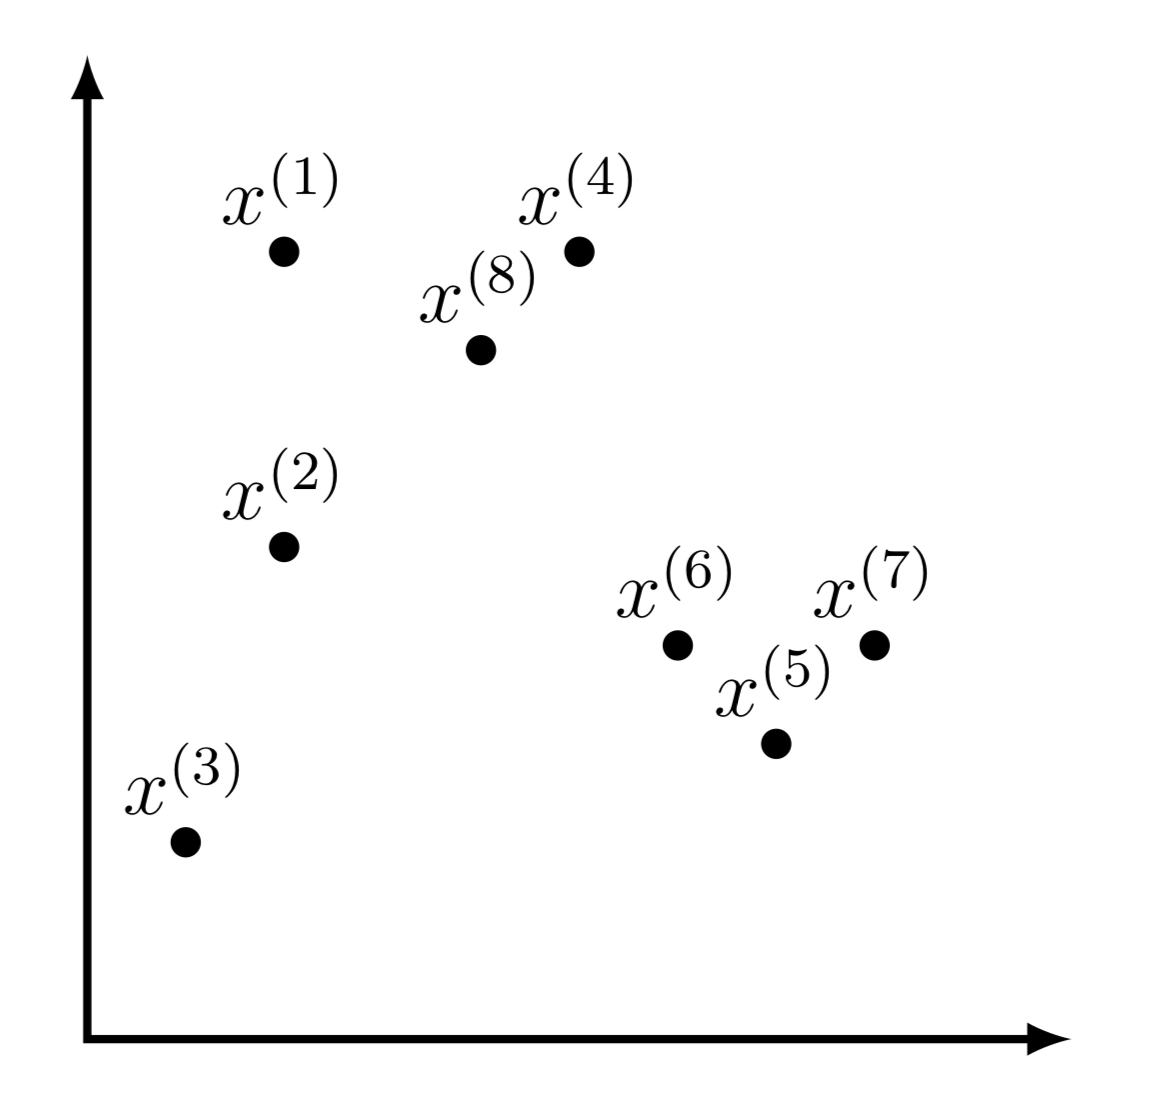
\includegraphics[width=0.4\linewidth]{media/images/kmeans.png}
\caption{Visualisierung des K-Means Datensatzes}
\end{figure}

\begin{subtask}[points=6,title={K-Means Algorithmus}]
Benutzen Sie den K-Means Algorithmus mit der Euklidischen Distanz um diese $8$ Datenpunkte in $K=3$ Cluster einzuteilen.
Die Cluster werden dabei als Cluster A, Cluster B und Cluster C beschrieben.
Nehmen Sie dabei an, dass die Clusterzentren $\mu_A^{(0)}, \mu_B^{(0)}, \mu_C^{(0)}$  mit den Punkten $x_3$, $x_6$ und $x_7$ initialisiert sind.
Führen Sie zwei Iterationen des K-Means Algorithmus durch und geben Sie die Koordinaten der Zentroide der Cluster an.

\begin{solution}
% Geben Sie hier Ihre Antwort an.
\end{solution}
\end{subtask}

\end{task}


\newpage
\begin{task}[credit=7]{Regressionsanalyse}
Gegeben sind folgende Datenpunkte:

\begin{table}[h]
\centering
\begin{tabular}{c|cccccccc}
\toprule
\textbf{x} & 1 & 3 & 4 & 6 & 8 & 9 & 11 & 14 \\ \hline
\textbf{y} & 1 & 2 & 4 & 4 & 5 & 7 & 8  & 9  \\
\bottomrule
\end{tabular}
\end{table}

\begin{figure}[h]
\centering
\caption{Veranschaulichung der Datenpunkte zur linearen Regression.}
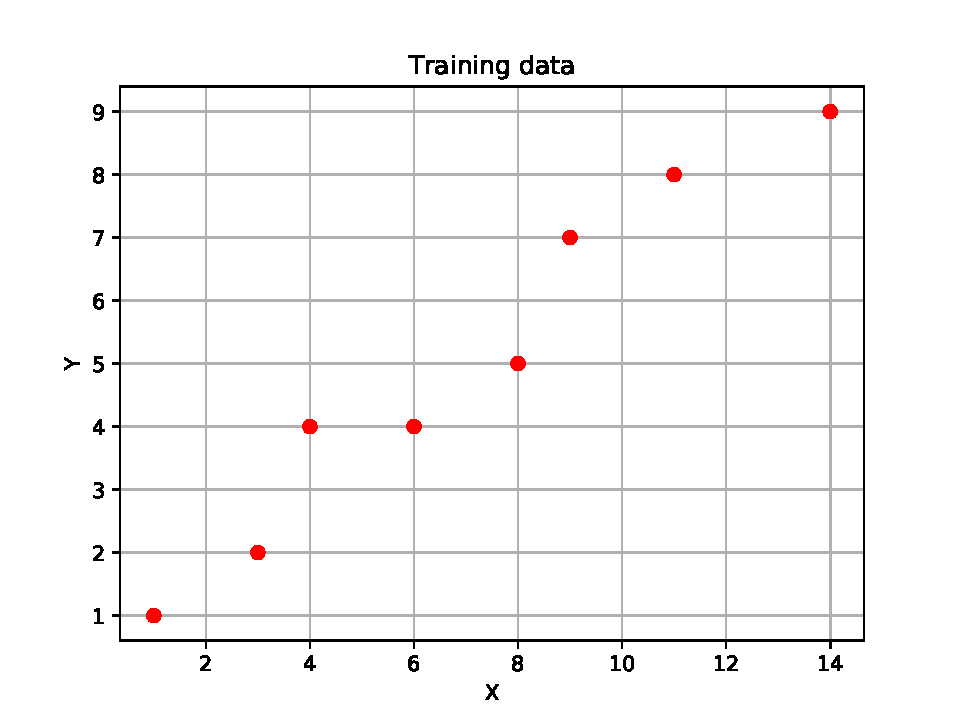
\includegraphics[width=0.5\linewidth]{media/images/data.pdf}
\end{figure}

Wir möchten eine Regression nach dem Prinzip der kleinsten Fehlrequadrate erstellen:

\begin{equation}
y =f(x)=\left \langle W, x  \right \rangle+b\,.
\end{equation}

Mit der Hilfe eines $(p+1)$-dimensionalen Vektors $\vec{x}=(1, x_1, \cdots , x_p)$ und $x \in \mathbb{R}^{1 \times p}$, können wir $b$ in dem Vektor $W$ codieren:

\begin{equation}
y =f(x)=\left \langle W^{'}, \vec{x}^{T}  \right \rangle,
\end{equation}

wobei hier $W^{'} \in \mathbb{R}^{2 \times 1}$ und $\vec{x} \in \mathbb{R}^{1 \times 2}$.

\begin{subtask}[title=Herleitung,points=5]
 Zeigen Sie, dass das optimale $W^{'}$:
\begin{equation}
W^{'} =  (\vec{X}^{T}\vec{X})^{-1}\vec{X}^{T}Y,
\end{equation}
entspricht, wobei $\vec{X} \in \mathbb{R}^{n \times 2}$ und $Y \in \mathbb{R}^{n \times 1}$.

\begin{solution}
% Geben Sie hier Ihre Antwort an.
\end{solution}
\end{subtask}


\begin{subtask}[title=Parameterbestimmung,points=2]
Berechnen Sie $W$ und $b$ für den gegebenen Punktdatensatz. Die Inverse $(\vec{X}^{T}\vec{X})^{-1}$ muss dabei nicht manuell berechnet werden.
\begin{solution}
% Geben Sie hier Ihre Antwort an.
\end{solution}
\end{subtask}
\end{task}


\end{document}
